% !TeX spellcheck = pt_br

%% abtex2-modelo-projeto-pesquisa.tex, v-1.9.5 laurocesar
%% Copyright 2012-2015 by abnTeX2 group at http://www.abntex.net.br/ 
%%
%% This work may be distributed and/or modified under the
%% conditions of the LaTeX Project Public License, either version 1.3
%% of this license or (at your option) any later version.
%% The latest version of this license is in
%%   http://www.latex-project.org/lppl.txt
%% and version 1.3 or later is part of all distributions of LaTeX
%% version 2005/12/01 or later.
%%
%% This work has the LPPL maintenance status `maintained'.
%% 
%% The Current Maintainer of this work is the abnTeX2 team, led
%% by Lauro César Araujo. Further information are available on 
%% http://www.abntex.net.br/
%%
%% This work consists of the files abntex2-modelo-projeto-pesquisa.tex
%% and abntex2-modelo-references.bib
%%

% ------------------------------------------------------------------------
% ------------------------------------------------------------------------
% - abnTeX2: Modelo de Projeto de pesquisa em conformidade com 
% - ABNT NBR 15287:2011 Informação e documentação - Projeto de pesquisa -
% - Apresentação 
% ------------------------------------------------------------------------ 
% ------------------------------------------------------------------------

\documentclass[
	% -- opções da classe memoir --
	12pt,				% tamanho da fonte
	openright,			% capítulos começam em pág ímpar (insere página vazia caso preciso)
	twoside,			% para impressão em verso e anverso. Oposto a oneside
	a4paper,			% tamanho do papel. 
	% -- opções da classe abntex2 --
	%chapter=TITLE,		% títulos de capítulos convertidos em letras maiúsculas
	%section=TITLE,		% títulos de seções convertidos em letras maiúsculas
	%subsection=TITLE,	% títulos de subseções convertidos em letras maiúsculas
	%subsubsection=TITLE,% títulos de subsubseções convertidos em letras maiúsculas
	% -- opções do pacote babel --
	english,			% idioma adicional para hifenização
	french,				% idioma adicional para hifenização
	spanish,			% idioma adicional para hifenização
	brazil,				% o último idioma é o principal do documento
	]{abntex2}

% ---
% -PACOTES
% ---

% ---
% Pacotes fundamentais 
% ---
\usepackage{lmodern}			% Usa a fonte Latin Modern
\usepackage[T1]{fontenc}		% Selecao de codigos de fonte.
\usepackage[utf8]{inputenc}		% Codificacao do documento (conversão automática dos acentos)
\usepackage{indentfirst}		% Indenta o primeiro parágrafo de cada seção.
\usepackage{color}				% Controle das cores
\usepackage{graphicx}			% Inclusão de gráficos
\usepackage{microtype} 			% para melhorias de justificação
% ---

% ---
% Pacotes adicionais, usados apenas no âmbito do Modelo Canônico do abnteX2
% ---
\usepackage{lipsum}				% para geração de dummy text
% ---

% ---
% Pacotes de citações
% ---
\usepackage[brazilian,hyperpageref]{backref}	 % Paginas com as citações na bibl
\usepackage[alf]{abntex2cite}	% Citações padrão ABNT

% --- 
% -CONFIGURAÇÕES DE PACOTES
% --- 

% ---
% Configurações do pacote backref
% Usado sem a opção hyperpageref de backref
\renewcommand{\backrefpagesname}{Citado na(s) página(s):~}
% Texto padrão antes do número das páginas
\renewcommand{\backref}{}
% Define os textos da citação
\renewcommand*{\backrefalt}[4]{
	\ifcase #1 %
		Nenhuma citação no texto.%
	\or
		Citado na página #2.%
	\else
		Citado #1 vezes nas páginas #2.%
	\fi}%
% ---

% ---
% Informações de dados para CAPA e FOLHA DE ROSTO
% ---
\titulo{Utilização de processamento natural de linguagem para abstração de logs}
\autor{Antonio Augusto Oliveira Viana Santos}
\local{Brasil}
\data{02-2016}
\instituicao{%
  Universidade Federal de Sergipe -- UFS
  \par
  PROCC - Programa de Pós-graduação em Ciência da Computação}
\tipotrabalho{Proposta de Mestrado}
% O preambulo deve conter o tipo do trabalho, o objetivo, 
% o nome da instituição e a área de concentração 
\preambulo{Proposta de Mestrado para PROCC}
% ---

% ---
% Configurações de aparência do PDF final

% alterando o aspecto da cor azul
\definecolor{blue}{RGB}{41,5,195}

% informações do PDF
\makeatletter
\hypersetup{
     	%pagebackref=true,
		pdftitle={\@title}, 
		pdfauthor={\@author},
    	pdfsubject={\imprimirpreambulo},
	    pdfcreator={LaTeX with abnTeX2},
		pdfkeywords={abnt}{latex}{abntex}{abntex2}{projeto de pesquisa}, 
		colorlinks=true,       		% false: boxed links; true: colored links
    	linkcolor=blue,          	% color of internal links
    	citecolor=blue,        		% color of links to bibliography
    	filecolor=magenta,      		% color of file links
		urlcolor=blue,
		bookmarksdepth=4
}
\makeatother
% --- 

% --- 
% Espaçamentos entre linhas e parágrafos 
% --- 

% O tamanho do parágrafo é dado por:
\setlength{\parindent}{1.3cm}

% Controle do espaçamento entre um parágrafo e outro:
\setlength{\parskip}{0.2cm}  % tente também \onelineskip

% ---
% compila o indice
% ---
\makeindex
% ---

% ----
% Início do documento
% ----
\begin{document}

% Seleciona o idioma do documento (conforme pacotes do babel)
%\selectlanguage{english}
\selectlanguage{brazil}

% Retira espaço extra obsoleto entre as frases.
\frenchspacing 

% ----------------------------------------------------------
% -ELEMENTOS PRÉ-TEXTUAIS
% ----------------------------------------------------------
% \pretextual

% ---
% Capa
% ---
\imprimircapa
% ---

% ---
% Folha de rosto
% ---
\imprimirfolhaderosto
% ---

% ---
% -NOTA DA ABNT NBR 15287:2011, p. 4:
%  ``Se exigido pela entidade, apresentar os dados curriculares do autor em
%     folha ou página distinta após a folha de rosto.''
% ---

% ---
% inserir lista de ilustrações
% ---
\pdfbookmark[0]{\listfigurename}{lof}
\listoffigures*
\cleardoublepage
% ---

% ---
% inserir lista de tabelas
% ---
%\pdfbookmark[0]{\listtablename}{lot}
%\listoftables*
%\cleardoublepage
% ---

% ---
% inserir lista de abreviaturas e siglas
% ---
%\begin{siglas}
%  \item[ABNT] Associação Brasileira de Normas Técnicas
%  \item[abnTeX] ABsurdas Normas para TeX
%\end{siglas}
% ---

% ---
% inserir lista de símbolos
% ---
%\begin{simbolos}
%  \item[$ \Gamma $] Letra grega Gama
%  \item[$ \Lambda $] Lambda
%  \item[$ \zeta $] Letra grega minúscula zeta
%  \item[$ \in $] Pertence
%\end{simbolos}
% ---

% ---
% inserir o sumario
% ---
\pdfbookmark[0]{\contentsname}{toc}
\tableofcontents*
\cleardoublepage
% ---


% ----------------------------------------------------------
% -ELEMENTOS TEXTUAIS
% ----------------------------------------------------------
\textual

% ----------------------------------------------------------
% Introdução
% ----------------------------------------------------------
\chapter[Contextualização]{Contextualização}

Durante os últimos anos, a segurança da informação tem sido uma grande preocupação para todos os usuários da Internet, devido aos diversos ataques que vem sendo perpetrados por meio dessa rede global. Por exemplo, segundo dados do CERT.br, o número total de notificações de incidentes de segurança superou a marca de um milhão em 2014, um aumento de mais de 200\% em relação ao ano anterior \cite{incidentes2015incidentes}. Para tentar mitigar esses incidentes a comunidade de segurança da informação vem desenvolvendo ferramentas e padrões para tornar os sistemas de informação mais seguros, de modo a dificultar o acesso a informações valiosas à pessoas não autorizadas. No entanto, os profissionais da área concordam em afirmar que não existe um sistema de segurança perfeito, apesar das técnicas e aplicações desenvolvidas \cite{dua2011data}.

Por esse motivo, as entidades que precisam de mais segurança optam por implantar Sistemas de Detecção de Intrusão (IDS, na sigla em inglês). O objetivo desses sistemas não é evitar que pessoas não autorizadas tenham acesso aos sistemas e/ou dados, mas detectar quando tais tentativas ocorram. Os primeiros trabalhos sobre IDSs são da década de 80 \cite{anderson1980computer, denning1987intrusion} e a partir de então vários trabalhos tem sido realizados para garantir que os IDSs possam sempre atender às demandas dos ambientes onde estão inseridos. Um dos principais desafios enfrentados por esses sistemas é o grande volume de dados que devem ser analisados, processados e exibidos de forma intuitiva para o usuário final \cite{big2013big, nassar2013secure}.

Além disso, estas tentativas de invasão através da Internet ou de outra rede de computadores, estão se tornando mais elaborados devido à constante criação de novos ataques ou de variantes dos existentes \cite{zuech2015intrusion}. Dessa maneira acredita-se que o futuro da detecção de intrusão depende de melhorias na detecção baseada em anomalias, visto que a detecção baseada em assinaturas oferece pouca capacidade de lidar com a velocidade com que novos ataques são gerados.

Para superar esse desafio, a comunidade acadêmica tem empreendido muitos esforços na busca de melhores arquiteturas para solução de detecção de intrusão, buscando, inclusive, inspiração (e técnicas) que obtiveram sucesso em outras áreas da computação. No entanto, para criar uma solução de IDS realmente inteligente, isto é, que possa detectar, de forma autônoma, vários ataques e que ofereça \emph{feedback} relevante para os seus usuários, devemos combinar várias tecnologias atualmente disponíveis (traçando um paralelo com \cite{schales2011stream}).

Com esse objetivo, buscou-se analisar diversos componentes que pudessem integrar uma arquitetura de IDS que atenda as necessidades mostradas, e julgados relevantes pela literatura recente. Esse estudo culminou na proposta apresentada na Figura \ref{fig:arquitetura-iids}. Essa figura mostra os componentes mais significativos para um sistema de IDS Inteligente (\emph{Inteligent IDS}, IIDS), os quais são:

\begin{figure}[ht]
	\centering
	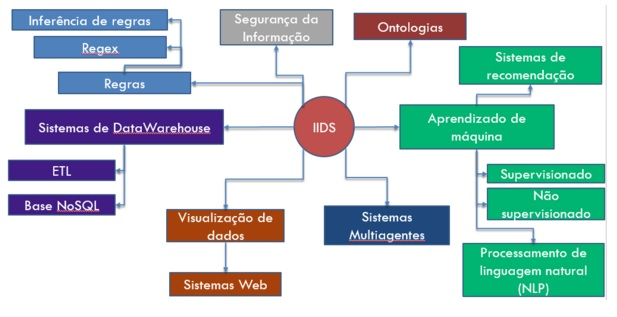
\includegraphics[width=.8\textwidth]{arquitetura-iids.jpg}
	\caption{Arquitetura idealizada para um IIDS}
	\label{fig:arquitetura-iids}
\end{figure}

\begin{itemize}
	
	\item \textbf{Aprendizado de máquina}: Técnicas de aprendizado de máquina (e de mineração de dados, de forma mais abrangente), são a base para um sistema de detecção de intrusão realmente inteligente, que ofereça suporta à detecção de anomalias com uma baixa taxa de falsos positivos;
	
	\item \textbf{Sistemas multiagentes}: O uso de sistemas multiagentes na modelagem do IDS oferece ganhos no processamento, e na inteligência do sistema. Além disso, a utilização de agentes móveis pode se mostrar de grande valia no cruzamento de informações de diferentes fontes;
	
	\item \textbf{Sistemas de \emph{data warehouse}}: O grande volume de informação gerado precisa ser analisado e armazenado da melhor maneira possível, levando em consideração: diversidade de dados, velocidade de aquisição de informações, volume de dados, facilidade para análise e visualização dos dados; acredita-se que o conjunto dessas características só pode ser alcançado através de um sistema distribuído; 
	
	\item \textbf{Visualização de dados}: Muito do \emph{feedback} oferecido pelo IDS deve ser visual, e com o grande volume de dados que é analisado, a maneira como esses dados são visualizados deve ser revista. Idealmente as informações devem ser exibidas de forma a agregar o máximo de informação possível, mas sem sobrecarregar o sistema visual do usuário;
	
	\item \textbf{Regras}: A base dos IDSs atuais não deve ser descartada. Detecção baseada em assinatura oferecem uma excelente taxa de verdadeiros positivos, e sua ampla utilização é prova inequívoca de sua capacidade de lidar (em parte) com o problema de detecção de intrusão. Acreditamos que, como em sistemas de detecção de \emph{SPAM}, o uso de técnicas baseadas em assinatura, usado em conjunto com outras técnicas, pode adicionar valor ao sistema;
	
	\item \textbf{Ontologias}: O uso de ontologias em sistemas de IDS pode trazer grandes avanços na questão semântica, permitindo um melhor entendimento dos impactos que podem ser causados pelos ataques. Enquanto alguns trabalhos já foram feitos focando no levantamento de requisitos para sistemas \cite{souag2012ontologies}, poucos ainda são focados no uso dessa técnica para os IDSs \cite{patel2013intrusion, sadighian2014ontids}.
	
\end{itemize}

Com base na arquitetura apresentada acima, em uma recente revisão da literatura conduzida durante o primeiro ano de mestrado (ainda a ser publicada), revisamos vários trabalhos que vem sendo desenvolvidos na área de detecção de intrusão usando os componentes elencados acima e identificamos que ainda existem diversos pontos de melhoria (nas soluções individuais e nas suas combinações).

Um dos pontos que nos chamou atenção durante essa revisão foi o uso de técnicas de aprendizado de máquina, e da variedade de possíveis aplicações que os pesquisadores têm encontrado dentro da área de detecção de intrusão. De interesse especial é a detecção de invasão através da análise de \emph{logs} de sistema (importante para \emph{compliance} de empresas, sendo requisito de padrões de segurança como o PCI DSS e a lei Sarbanes-Oxley \cite{prakhar2012log}).

O padrão para a geração de \emph{logs} em ambientes UNIX\texttrademark é o \emph{syslog}. As mensagens de \emph{log} do formato syslog são em texto plano e, em sua maioria, escritas em linguagem corrente. O uso de linguagem corrente torna esses \emph{logs} fáceis para interpretar por humanos, mas difíceis de serem analisados por máquinas. O uso de técnicas de processamento natural de linguagem (uma sub-área do aprendizado de máquina) pode ser usada para extrair informações das entradas de logs. Para isso focaremos em técnicas de extração e recuperação de informação \cite{bird2009natural,manning2008introduction}.

A análise de \emph{logs} é feita hoje em dia é feita ou manualmente (gerando padrões de texto de forma manual através do uso de expressões regulares - \emph{regex}) onde é possível a extração das ``entidades''\footnote{Por entidades nos referimos aos hosts, ips, usuários, etc, que são referidos em uma linha de log} que compõe uma linha de \emph{log}, ou de forma automática, onde são agrupadas linhas similares (com variados graus de sucesso), mas sem conseguir discernir os componentes de cada linha.

A ideia do uso da linguagem natural é permitir a geração automática de expressões regulares que consigam, não só agrupar linhas de \emph{logs} similares, mas que também possam detectar as entidades presentes nessas linhas, e correlacioná-las entre linhas de origens diferentes (isto é, saber que dois campos em entradas de \emph{logs} diferentes se referem à entidade usuário).

Além da aplicabilidade para a análise de \emph{logs}, acreditamos que o uso do processamento natural de linguagem em registros gerados por computadores pode gerar um impacto positivo na área de armazenamento de dados. Esse ganho é alcançado principalmente quando consideramos o cenário de aquisição de dados heterogêneos, necessário para um melhor desempenho dos IDSs \cite{zuech2015intrusion}.

Essa proposta é dividida da seguinte forma: no Capítulo \ref{chap:referencial} apresentaremos o referencial teórico de suporte ao nosso trabalho; no Capítulo \ref{chap:proposta} apresentaremos nossa proposta e seus impactos, inicialmente, em alto nível, e a seguir serão mostrados alguns dos detalhes técnicos do que esperamos alcançar com nosso trabalho; por último, no Capítulo \ref{chap:cronograma} mostraremos um cronograma das nossas atividades para o próximo ano.

\subsection{Objetivos}

O objetivo geral deste trabalho é o de estudar técnicas de Processamento Natural de Linguagem (PNL; NLP na sigla em inglês) que possam ser aplicadas as técnicas de abstração de logs, permitindo a identificação de entidades dentro dos \emph{logs}, gerando melhores abstrações.

Como objetivos específicos podemos citar:
\begin{itemize}
	\item{\textbf{Revisar o estado da arte}} Avaliar o estado da arte das soluções de abstração de \emph{logs} e de processamento natural de linguagem, dentro da comunidade acadêmica;

	\item{\textbf{Pesquisar ferramentas}} Estudar as ferramentas que pretendemos utilizar dentro de nosso trabalho (especificamente a biblioteca NLTK \cite{bird2009natural}.)
	
	\item{\textbf{Definir política de avaliação}} Definir uma política de avaliação de nossa solução, para podermos identificar melhoras no nosso trabalho, e poder gerarmos comparações com outros trabalhos publicados;
	
	\item{\textbf{Implementar um produto de software}} Implementar um produto de software usando as técnicas estudadas acima;
	
	\item{\textbf{Analisar desempenho da solução implementada}} Usar a política de avaliação definida para verificar ganhos da nossa solução;
	
	\item{\textbf{Publicação dos resultados encontrados}} Compartilhar os resultados encontrados com a comunidade acadêmica, através da publicação de artigos em congressos com Qualis, e  da elaboração de uma dissertação de mestrado, ou da compilação de artigos publicados;
	
\end{itemize}

Com essa abordagem nos esperamos alcançar alguns objetivos que não encontramos em nenhum outro ponto da literatura:

\begin{itemize}
	\item Definir uma política de avaliação da capacidade de abstração de \emph{logs}, que pode ser usado para avaliar novas ferramentas;
	\item Definir uma nova forma de abstração de \emph{logs}, que consegue detectar o tipo de entidade presente nos \emph{logs};
\end{itemize}

\subsection{Trabalhos relacionados}
- O que os outros fizeram

\section{Metodologia}

Vamos trabalhar com uma abordagem incremental, resolvendo problemas aos poucos.

Num primeiro momento queremos conseguir extrair os ``templates'' de \emph{logs} de um único programa (já feito por alguns pesquisadores \cite{nagappan2010abstracting}). Em seguida queremos extrair, desse único tipo de \emph{log}, as entidades que o compõe, de forma a já correlaciona-las (isto é, saber que dois nomes, referem-se a usuários, por exemplo). Esse é uma de nossas principais contribuições, por não encontramos nenhum trabalho que faça esse tipo de geração de forma automática.

Como última etapa queremos correlacionar as entidades através de diferentes tipos de \emph{logs}, ou seja, saber quais campos, de diferentes tipos de \emph{logs}, se referem a um usuário ou a um \emph{host}, por exemplo.

\subsection{Analise de desempenho}

% ----------------------------------------------------------
% Capitulo de textual  
% ----------------------------------------------------------
\chapter{Referencial Teórico}\label{chap:referencial}

Nesta seção apresentaremos alguns trabalhos que vem sendo executados na área de detecção de intrusões com uso de técnicas de aprendizado de máquina, trabalhos relacionados a abstração de \emph{logs}, e as realizações atuais sobre o processamento natural de linguagem. No tocante ao uso de aprendizado de máquina, vê-se que os trabalhos não se restringem somente à detecção de anomalias, com várias outras aplicações sendo realizadas. Quanto à abstração de \emph{logs}, vemos que os trabalhos se concentram somente em encontrar padrões de texto, e não na recuperação de entidades, como propomos. Por último, as técnicas de processamento natural de linguagem vem mostrando um rápido crescimento e expandindo sua aplicabilidade.

\section{Aprendizado de máquina}\title{sec:aprendizado_de_maquina}
O uso de técnicas de aprendizado de máquina começou a ser explorada na área de detecção de intrusões focando em melhorias na detecção de anomalias em IDSs, visto que a maioria dos sistemas hoje usam técnicas de detecção por assinatura, o que restringe sua ação para detecção de variações de ataques existentes, ou mesmo de novos ataques. Essas técnicas, e a mineração de dados, de forma geral, tem apresentado bons resultados nesse sentido \cite{dua2011data, yen2013beehive, zomlot2013aiding, ganapathy2012intelligent, li2013automatic, joseph2012machine}.

Em \cite{yen2013beehive} é apresentado um trabalho com o uso de técnicas de clusterização (uma variação do algoritmo K-means\cite{ball1967clustering}), para a detecção de possíveis infecções de \emph{malwares} em sistemas conectados à Internet através da análise de \emph{logs} de \emph{proxies}, servidores de VPN, DHCP e controladores de domínio Microsoft Windows \texttrademark. Os resultados apresentados nesse trabalho são extremamente relevantes e encorajadores, por duas razões: i) o sistema conseguiu identificar mais de 750 incidentes, dos quais apenas 8 haviam sido detectados anteriormente por sistemas de segurança já usados na empresa onde o estudo foi realizado; ii) o trabalho é feito com um volume grande de informações (cerca de 1 Tb/dia), claramente um desafio relacionado à \emph{Big Data}. No trabalho são mostradas técnicas para a redução do volume de dados e para a seleção de \emph{features} para análise.

Ainda no campo de detecção de anomalias, em \cite{li2013automatic} bons resultados são alcançados através da combinação de técnicas diferentes de aprendizado de máquina. Nesse trabalho são apresentados dois algoritmos aplicados sequencialmente: o primeiro usado para criar meta-eventos, e o segundo para classificação, usando esses meta-eventos (ao invés dos eventos em si). Nesse trabalho são usados os algoritmos SOM \cite{kohonen1989self}, para gerar os meta-eventos e o DBSCAN \cite{ester1996density}, para a agregação dos meta-eventos.

Mas, além da detecção de anomalias, outro campo que tem recebido muita pesquisa na academia é o uso de mineração de dados para lidar com o grande volume de alertas gerados pelos IDSs baseados em regras usados atualmente. O trabalho apresentado em \cite{zomlot2013aiding}, por exemplo, utiliza a aprendizagem de máquina para tentar priorizar os incidentes: um modelo aprende a opinião de analistas sobre a prioridade dos alertas, e esse conhecimento, posteriormente, é replicado pelo sistema, priorizando automaticamente os alertas .

Outros trabalhos tentam preencher a lacuna na correlação de eventos de segurança, de forma a identificar a relação entre eventos distintos \cite{smith2008using, stroeh2013approach}.

\section{Abstração de logs}\title{sec:informacao}
- Mais detalhes

\subsection{Repositório de logs que vão ser analisados}

\section{Processamento natural de linguagem}

A área de mineração de textos, em especial a área de extração de informações, vem realizando trabalhos similares ao nosso, mas em um outro contexto \cite{duque2012processo, matos2010environment}.

\subsection{Bibliotecas de processamento natural de linguagem}

Nosso objetivo não é desenvolver um novo paradigma para o processamento natural de linguagem. Por isso iremos fazer uso de bibliotecas de programação já existentes, que forneçam suporte as técnicas que pretendemos utilizar. Para isso planejamos usar a biblioteca NLTK (Ferramentas de Linguagem Natural, na sigla em inglês) \cite{bird2009natural}. Essa biblioteca funciona em conjunto com a linguagem de programação Python.

A escolha dessa biblioteca foi feita levando em consideração os seguintes pontos:

\begin{itemize}
	\item Biblioteca distribuída livremente (sob licença Open-Source), o que facilita a reprodutibilidade do trabalho;
	\item Documentação ampla, facilitando seu uso;
	\item Utilização da linguagem Python (de domínio do mestrando);
\end{itemize}

Além disso, a linguagem Python, por si só, possui mais algumas vantagens, que a tornam interessante para o desenvolvimento de uma solução de software completa:
\begin{itemize}
	\item Outras bibliotecas que dão suporte a diversas técnicas de aprendizado de máquina (que podem ser necessárias durante o desenvolvimento do trabalho);
	\item Suporte para a criação de uma solução de software completa (suporte à conectividade à banco de dados, e ao desenvolvimento de aplicações Web, por exemplo);
	\item Facilidade de conectividade com outras linguagens de programação (\emph{bindings});
\end{itemize}

\chapter{Utilização de processamento natural de linguagem para abstração de logs}\label{chap:proposta}

Nessa seção trataremos do caso especial especial da análise de \emph{logs} (como parte de IDS de \emph{host}), nesse cenário o caso mais comum para as fontes de dados são as entradas não estruturadas. Os arquivos de \emph{logs}, normalmente, tentam ser de mais fácil leitura para os humanos, em detrimento da facilidade de processamento, gerando problemas para serem analisados automaticamente por computadores. Trabalhos como \cite{vaarandi2003data, nagappan2010abstracting} tentam agrupar tipos parecidos de \emph{logs} (gerando \emph{"templates"} usando expressões regulares ou \emph{wildcards}).

Nesse sentido o uso das técnicas de processamento de linguagem natural (PNL; NLP na sigla em inglês) podem ajudar a evoluir esse conceito. Podemos usar o PNL para encontrar o significado de uma frase (positivo ou negativo) e tentar encontrar as entidades referenciadas em uma dada linha de \emph{log} (usuário, IP de origem, sistema impactado, etc). Podemos ainda correlacionar automaticamente o mesmo tipo de entidade em diferentes \emph{logs} (mesmo entre aplicações diferentes).  Nesse sentido fomos inspirados pelos trabalhos exibidos em \cite{matos2010environment, duque2012processo}.

Esse avanço também pode gerar impactos no processo de consolidação de dados, um grande desafio existente hoje, não só nos IDSs como também para qualquer sistema de \emph{Big Data} \cite{zuech2015intrusion}. Em especial, se a classificação automática de entidades puder se feita de forma online (durante o  \emph{streaming} de dados), podemos começar a trabalhar de forma muito mais rápida, e com menor tempo de reação, para novos ataques, através da integração continua de dados.

\section{Proposta de Implementação}\label{sec:implementacao}

A nossa ideia é desenvolver um algoritmo que permite a detecção de padrões em \emph{logs} de sistemas. A principal diferença de nossa abordagem para as que existem hoje em dia, é que não queremos somente agrupar \emph{logs} similares, como em \cite{vaarandi2003data}, mas também detetar ``entidades'' dentro dos \emph{logs}, através de técnicas de mineração de texto.

A extração de entidades vai permitir a aplicação de técnicas de aprendizado de máquina em todo a massa de \emph{logs}, visto que, para um melhor desempenho de técnicas de aprendizado de máquina é necessário que as entidades estejam identificadas.

Por exemplo, observando-se as seguintes linhas de \emph{log}:

{\tiny
	\begin{verbatim}
	alien12 sshd[16448]: Invalid user developer from 116.255.160.35
	alien12 sshd[16448]: pam_unix(sshd:auth): check pass; user unknown
	alien12 sshd[16448]: pam_unix(sshd:auth): authentication failure; logname= uid=0 
	euid=0 tty=ssh ruser= rhost=116.255.160.35 
	alien12 sshd[16448]: Failed password for invalid user developer from 116.255.160.35 port 33732 ssh2
	alien12 sshd[17551]: Invalid user developer from 116.255.160.35
	alien12 sshd[17551]: pam_unix(sshd:auth): check pass; user unknown
	alien12 sshd[17551]: pam_unix(sshd:auth): authentication failure; logname= uid=0 euid=0 
	tty=ssh ruser= rhost=116.255.160.35 
	alien12 sshd[17551]: Failed password for invalid user developer from 116.255.160.35 port 34084 ssh2
	alien12 sshd[18758]: Invalid user developer from 116.255.160.35
	\end{verbatim}
}

nós pretendemos extrair as seguintes informações:

\begin{itemize}
	\item \textbf{user}: developer	
	\item \textbf{src\_ip}: 116.255.160.35	
	\item \textbf{port}: 33732, 34084	
	\item \textbf{uid}: 0	
	\item \textbf{euid}: 0	
	\item \textbf{tty}: ssh 
\end{itemize}

Explicar o que queremos extrair, e correlacionar. Falando como no exemplo

Observe que essas informações foram extraídas de um único tipo de evento (\emph{logs} do servidor sshd), mas é nossa intenção que as entidades possam ser correlacionadas entre entradas de \emph{logs} de programas diferentes.

DAR EXEMPLO DE CORRELAÇÃO ENTRE LOGS DIFERENTES

Além disso queremos usar informações do texto para melhor classificar as entidades.
Por exemplo, observe as entradas de log abaixo:

{\tiny
\begin{verbatim}
refused connect from 192.168.0.1:1231 to procedure ypproc_domain_nonack 
connect to 192.168.0.1:25: Connection timed out
\end{verbatim}
}

Enquanto a entidade 192.168.0.1, aparece nas duas entradas de logs (e nos dois casos ela é um IP), ela tem contextos diferentes. No primeiro caso a entidade é um IP de origem (isto é, está originando a ação), no segundo caso ela é o IP de destino (recebe uma ação). Esse tipo de diferença é importante durante o processo de análise de logs e poder servir de insumo para tomada de decisões.

Nesse caso, observe que o tipo da entidade, é indicada pelo contexto do \emph{log}, e as indicações do texto (a precedência das palavras \emph{from} e \emph{to}), indicam o tipo de cada uma das entidades.

\cite{bird2009natural}

\subsection{Criação de implementação}

- Análise de desempenho

\chapter{Cronograma}\label{chap:cronograma}

% ---
% Finaliza a parte no bookmark do PDF
% para que se inicie o bookmark na raiz
% e adiciona espaço de parte no Sumário
% ---
\phantompart

% ---
% Conclusão
% ---
%\chapter*[Considerações finais]{Considerações finais}
%\addcontentsline{toc}{chapter}{Considerações finais}

% ----------------------------------------------------------
% - ELEMENTOS PÓS-TEXTUAIS
% ----------------------------------------------------------
\postextual

% ----------------------------------------------------------
% Referências bibliográficas
% ----------------------------------------------------------
\bibliography{bibliografia}

% ----------------------------------------------------------
% Glossário
% ----------------------------------------------------------
%
% Consulte o manual da classe abntex2 para orientações sobre o glossário.
%
%\glossar

% ----------------------------------------------------------
% Apêndices
% ----------------------------------------------------------

%---------------------------------------------------------------------
% -INDICE REMISSIVO
%---------------------------------------------------------------------

\phantompart

\printindex


\end{document}
